\documentclass[12pt, notitlepage]{article}
\usepackage[utf8]{inputenc}
\usepackage{multicol}
\usepackage{multirow}
\usepackage[margin=0.5in]{geometry}
\usepackage[utf8]{inputenc}
\usepackage{tikz}
\usepackage{graphicx}
\graphicspath{{./images/}}
\usepackage{soul}
\usepackage{listings}
\usepackage{xcolor}
\usetikzlibrary{arrows}
\usepackage{mathtools}
\usepackage{amsmath}
\usepackage{pgfplots}
\pgfplotsset{compat=1.8}
\usepgfplotslibrary{statistics}
\usepackage{float}
\usepackage{tabto}
\usepackage{caption}
\usepackage{diagbox}
\usepackage{hyperref}

\title{CSE 145 - Final Project}
\author{Daniel Xiong (dxiong5@ucsc.edu)\\
		Nyi Nyi "Scott" Zin (nzin@ucsc.edu)}
\date{}

\begin{document}
\maketitle

\section{Abstract}
Data Mining and Natural Language Processing are two rapidly developing fields, and the intersection of these can yield interesting projects. In this report, we explain how we utilized Data Mining and NLP concepts to try and predict the stock price of Tesla Inc. using the tweets of its outspoken CEO, Elon Musk. Examples of relevant projects are provided and major challenges and open issues are identified.

\section{Introduction}
The goal of this project is to attempt to predict whether Tesla's (\texttt{\$TSLA}) stock price will go up or down based on Elon Musk's tweets; in other words, this is a class prediction problem and we want to classify Musk's tweets. To achieve this goal, we first collected the data: \texttt{TSLA} stock history from its Initial Public Offering (IPO) in 2010 to May 26, 2020 and Elon Musk's tweets dating from his first tweet in 2011 to May 26, 2020. We then pre-processed the data and created visualizations to better understand what we were working with. Next, we utilized sentiment analysis, a NLP technique that gives each tweet a positive or negative sentiment score. Finally, we used the tweet sentiments along with the stock data and implemented a few different predictive classification models: a neural network, decision tree, random forest, and naïve bayes.

\section{Tools Used}
This assignment was completed using Python 3.7 (\texttt{sklearn}, \texttt{keras}, \texttt{pandas}, \texttt{matplotlib}). Refer to the README to find instructions on how to run the code.

\section{Data}
\subsection{Data Collection}
We collected \texttt{\$TSLA} stock history by downloading it directly from Yahoo! Finance. The raw data contains the date, price at open and close, and highs and lows of the day. We store this data in \texttt{/src/data/TSLA.csv}. \\\\
Elon Musk's tweets were scraped using Python's \texttt{GetOldTweets3} package. We first tried using Twitter's API directly, but the API doesn't allow us to scrape tweets older than a week. \texttt{GetOldTweets3} is a package that doesn't have such limitations, allowing us to obtain all of Musk's 9785 tweets. The raw data, which contains a tweet ID, permalink to the tweet, Twitter handles, tweet contents, date, retweets, and favorites, is stored in \texttt{/src/data/TSLA.csv}.

\subsection{Data Pre-processing for Sentiment Analysis}
Elon Musk's tweets needed substantive pre-processing for sentiment analysis. The initial pre-processing step was to remove non-English characters, such as Chinese and Russian, remove tweets that were just pictures with no text caption, and remove hyperlinks. Next, to prepare the dataset for sentiment analysis, we strip all punctuation (!, ?, \$, etc.), numbers, and excessive whitespace. We do this because these characters do not have any inherent sentiment, so it would not contribute to the sentiment analysis task. The processed tweets are stored in \texttt{/src/data/elon\_musk\_tweets\_processed.csv}.

\subsection{Sentiment Analysis}
For sentiment analysis, we used Python's \texttt{TextBlob} package. \texttt{TextBlob} uses WordNet, a lexical database of words and their semantic relationships that is designed to be used for NLP tasks. \texttt{TextBlob} uses WordNet, a pre-trained Part-of-Speech tagging model, and a pre-trained sentiment model to output a polarity and subjectivity measure. We focused on the polarity measure, which is a number in the range $[-1,1]$, where $-1$ is a negative sentiment and $1$ is a positive sentiment. Each tweet in our dataset was given a polarity measure, and is stored in \texttt{/src/data/elon\_musk\_tweets\_sentiments.csv}.

\subsection{Data Understanding and Analysis}
\textbf{Figure 1} shows a bar graph that shows the number of tweets by Elon Musk per year since 2010. The bar for 2020 is only half of that of 2019, but that is because we are only halfway through the year. One reason for the exponential increase in tweets per year can be simply due to the increased popularity of Twitter as a platform, or because of the success of Musk's companies.\\\\
\textbf{Figure 2} shows a bar graph that shows the distribution of whether the stock closed higher (moved up) or lower (moved down) compared to when it opened for the day. As we can see in the graph, our data is extremely balanced, with an even distribution of both cases.\\\\
\textbf{Figure 3} shows a bar graph that shows the distribution of the results from the sentiment analysis. We labeled tweets as either negative, neutral, or positive using the following function,
\[ Label(p) = \begin{cases} 
Negative & p < -0.1 \\
Neutral & -0.1 \leq p \leq 0.1\\
Positive & p > 0.1\\
\end{cases}
\]\\
where $p$ is the polarity value for a tweet. From the graph, we see that a large portion of Elon Musk's tweets have a neutral sentiment.\\\\
\textbf{Figure 4} and \textbf{Figure 5} show the sentiments and \texttt{\$TSLA} stock movement over the time period of June 2017, respectively. These graphs are meant to act as a visual comparison between sentiments and stock movement.
\begin{figure}[H]
	\centering
	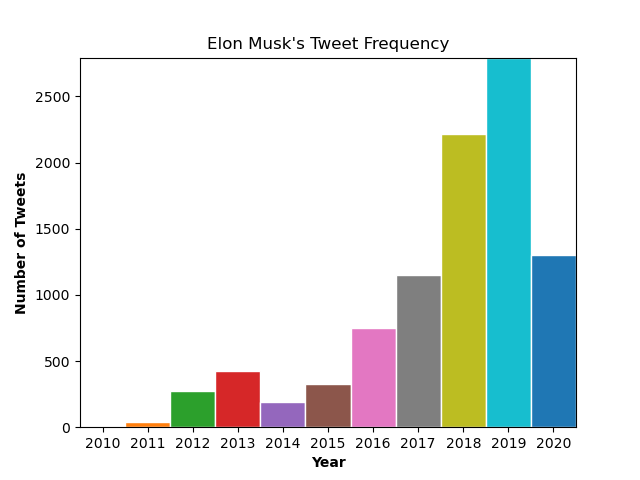
\includegraphics[scale=0.8]{images/Frequency.png}
	\caption{Frequency of tweets per Year}
	\label{fig:F}
\end{figure}
\begin{figure}[H]
	\centering
	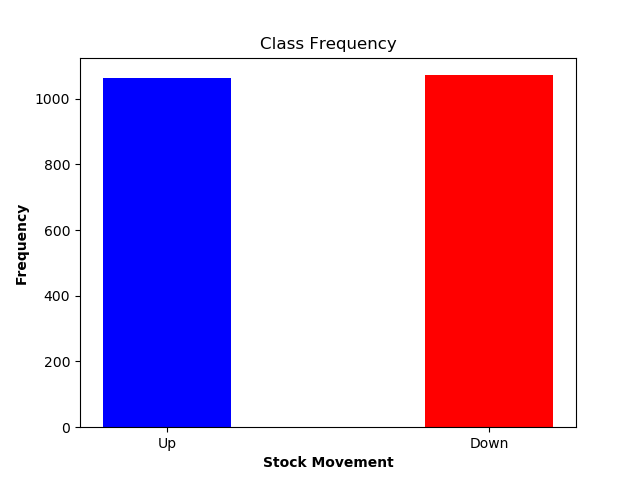
\includegraphics[scale=0.8]{images/Class_Distribution.png}
	\caption{Stock Movement Class Frequency}
	\label{fig:SM}
\end{figure}
\begin{figure}[H]
	\centering
	\includegraphics[scale=0.8]{images/sentiment_distribution.png}
	\caption{Sentiment Distribution}
	\label{fig:SD}
\end{figure}
\begin{figure}[H]
	\centering
	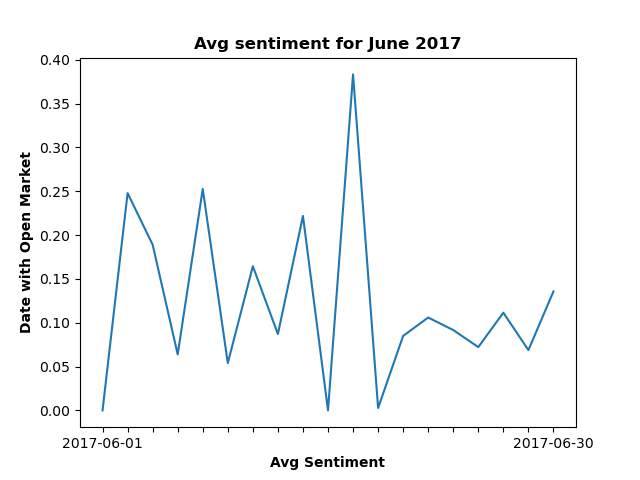
\includegraphics[scale=0.8]{images/sentiment_overtime.png}
	\caption{Sentiment distribution for June 2017}
	\label{fig:SO}
\end{figure}
\begin{figure}[H]
	\centering
	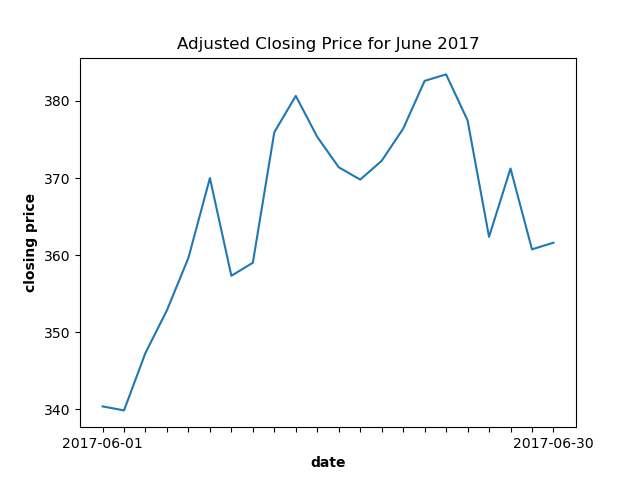
\includegraphics[scale=0.8]{images/stock_overtime.png}
	\caption{Stock Price for June 2017}
	\label{fig:SP}
\end{figure}

\section{Prediction Models}
We implemented 4 different predictive classification models: a neural network, decision tree, random forest, and naïve bayes.
\subsection{Neural Network}
The first type of predictive model we chose was a simple feed-forward neural network. We used \texttt{keras}'s \texttt{Sequential} model. The model architecture was 1x8x8x4x1, where there was a single input node, 3 fully connected hidden layers, and a single node as the output node. We used Binary Cross Entropy as our loss function, the Adam optimizer, 20 epochs, and the sigmoid function as the activation function for the output node. The model was trained and validated using a 75/25 training and test split of the dataset. \\\\
On the training data, the model achieved an accuracy of 0.5055. \textbf{Figure 6} shows the accuracy over the 20 epochs. The plot shows a very jagged line, which usually means that the model doesn't really have anything to learn.\\\\
\begin{figure}[H]
	\centering
	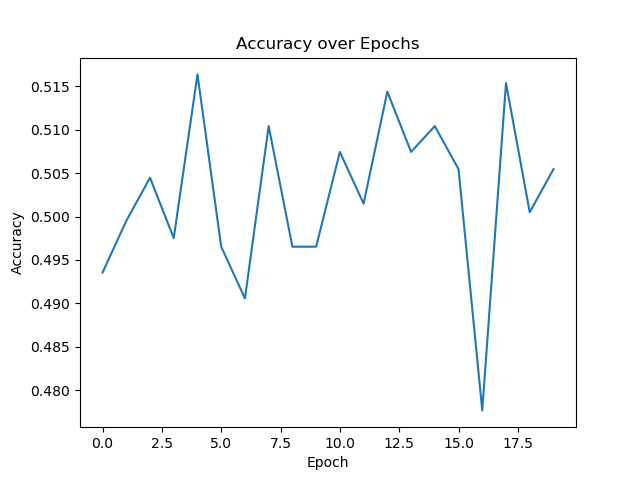
\includegraphics[scale=0.8]{images/neural_net_accuracy.png}
	\caption{Accuracy over Epochs}
	\label{fig:NN}
\end{figure}
On the validation data, the neural network achieved an accuracy of 0.5238. We wanted to make take other metrics into account, so we created a confusion matrix and calculated the precision, recall, and F1 scores.
\begin{table}[H]
	\caption{Neural Network Confusion Matrix}
	\centering
	\begin{tabular}{|c|c|c|}
		\hline
		\diagbox[width=11em]{Actual}{Predicted} & Negative & Positive \\
		\hline
		Negative & 34 & 130 \\
		\hline
		Positive & 30 & 142 \\
		\hline
	\end{tabular}
\end{table}
\begin{table}[H]
	\centering
	\begin{tabular}{|c|c|c|}
		\hline
		Precision & Recall & F1 \\
		\hline
		0.5221 & 0.8256 & 0.6396 \\
		\hline
	\end{tabular}
\end{table}
The precision is relatively low, at 0.5221, which means that about half of the 'stock goes up' classifications are wrong. Our recall score is relatively high, meaning that our model predicts a high percentage of true positives (stock goes up) out of all of the actual positives. 
\subsection{Decision Tree}
Given the poor performance of the neural network, we decided to use a simpler model: a decision tree. The decision tree model used is \texttt{sklearn}'s \texttt{DecisionTreeClassifier} model. The hyper-parameters that we tuned were: Gini impurity to measure the quality and a max tree depth of 3. Like the neural network model, the decision tree was trained and tested with a 75/25 split on the dataset. \\\\
The decision tree model got a test accuracy of 0.5179; the tree is shown in \textbf{Figure 7}.
\begin{figure}[H]
	\centering
	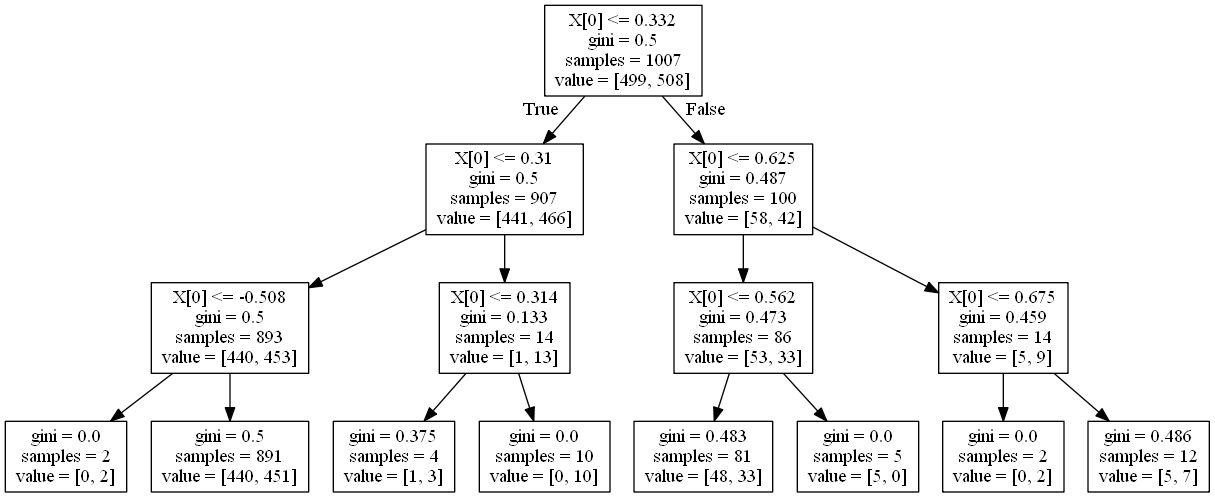
\includegraphics[scale=0.45]{images/tree.png}
	\caption{Decision Tree}
	\label{fig:DT}
\end{figure}
We created a confusion matrix and calculated the precision, recall, and F1 scores.
\begin{table}[H]
	\caption{Decision Tree Confusion Matrix}
	\centering
	\begin{tabular}{|c|c|c|}
		\hline
		\diagbox[width=11em]{Actual}{Predicted} & Negative & Positive \\
		\hline
		Negative & 14 & 150 \\
		\hline
		Positive & 12 & 162 \\
		\hline
	\end{tabular}
\end{table}
\begin{table}[H]
	\centering
	\begin{tabular}{|c|c|c|}
		\hline
		Precision & Recall & F1 \\
		\hline
		0.5161 & 0.9302 & 0.6639 \\
		\hline
	\end{tabular}
\end{table}
The precision, recall, and F1 scores very closely resemble the scores from the neural network model. Much like the neural network, the decision tree has a high recall and relatively low precision. 
\subsection{Random Forest}
We decided to implement a random forest model to try and improve upon the decision tree model. The random forest model used is \texttt{sklearn}'s \texttt{RandomForestClassifier} model. We tuned the hyper-parameters to be a max depth of 3 and the max number of leaf nodes to be 5. This model gave us an accuracy of 0.5268 on the test dataset. We created a confusion matrix and calculated the precision, recall, and F1 scores.
\begin{table}[H]
	\caption{Random Forest Confusion Matrix}
	\centering
	\begin{tabular}{|c|c|c|}
		\hline
		\diagbox[width=11em]{Actual}{Predicted} & Negative & Positive \\
		\hline
		Negative & 59 & 105 \\
		\hline
		Positive & 54 & 118 \\
		\hline
	\end{tabular}
\end{table}
\begin{table}[H]
	\centering
	\begin{tabular}{|c|c|c|}
		\hline
		Precision & Recall & F1 \\
		\hline
		0.5291 & 0.6860 & 0.5975 \\
		\hline
	\end{tabular}
\end{table}
The accuracy for the random forest model was barely better than that of the decision tree model. The precision is about the same as the decision tree model, but the recall is lower.
\subsection{Naïve Bayes}
We chose to include a naïve bayes classifier model because we wanted to see how a probabilistic model would perform. This model is implemented using \texttt{sklearn}'s \texttt{GaussianNB} Gaussian Naïve Bayes classifier. The model produced an accuracy of 0.5089 on the test data. We created a confusion matrix and calculated the precision, recall, and F1 scores.
\begin{table}[H]
	\caption{Naïve Bayes Confusion Matrix}
	\centering
	\begin{tabular}{|c|c|c|}
		\hline
		\diagbox[width=11em]{Actual}{Predicted} & Negative & Positive \\
		\hline
		Negative & 53 & 111 \\
		\hline
		Positive & 54 & 118 \\
		\hline
	\end{tabular}
\end{table}
\begin{table}[H]
	\centering
	\begin{tabular}{|c|c|c|}
		\hline
		Precision & Recall & F1 \\
		\hline
		0.5153 & 0.6860 & 0.5885 \\
		\hline
	\end{tabular}
\end{table}
We can see that this naïve bayes classifier model gave very similar scores in comparison to the random forest model.
\section{Analysis and Conclusion}
All of our models performed poorly, with accuracies of 50.55\%, 51.79\%, 52.68\%, and 50.89\% on the neural network, decision tree, random forest, and naïve bayes models respectively. The data was balanced, and the training and test data was shuffled to mitigate any patterns in the data ordering. \\\\
The most probable conclusion we can draw from our model performance is that there is no correlation between Elon Musk's tweet sentiment and Tesla's stock performance. There are some edge cases however, such as when Musk tweeted "Tesla stock price is too high imo" and \texttt{\$TSLA} subsequently dropped 10\%. This tweet can be considered an edge case because Musk rarely explicitly mentions \texttt{\$TSLA} stock price.\\\\
All in all, even though Elon Musk is outspoken and has tweeted some pretty controversial things, Wall Street simply does not care and will only care about earnings reports and profits. 

\section{Related Work}
One related project we found ran a sentiment analysis on Donald Trump's tweets, and try to predict the performance of the S\&P 500 index. \href{https://towardsdatascience.com/covfefe-nlp-do-trumps-tweets-move-the-stock-market-42a83ab17fea}{Link Here}\\\\
Another related project we found used sentiment analysis on a daily corpus of tweets to try and predict the Dow Jones Industrial Average. \href{http://cs229.stanford.edu/proj2011/GoelMittal-StockMarketPredictionUsingTwitterSentimentAnalysis.pdf}{Link Here}


\end{document}